% Options for packages loaded elsewhere
\PassOptionsToPackage{unicode}{hyperref}
\PassOptionsToPackage{hyphens}{url}
\PassOptionsToPackage{dvipsnames,svgnames,x11names}{xcolor}
%
\documentclass[
  letterpaper,
  DIV=11,
  numbers=noendperiod]{scrartcl}

\usepackage{amsmath,amssymb}
\usepackage{iftex}
\ifPDFTeX
  \usepackage[T1]{fontenc}
  \usepackage[utf8]{inputenc}
  \usepackage{textcomp} % provide euro and other symbols
\else % if luatex or xetex
  \usepackage{unicode-math}
  \defaultfontfeatures{Scale=MatchLowercase}
  \defaultfontfeatures[\rmfamily]{Ligatures=TeX,Scale=1}
\fi
\usepackage{lmodern}
\ifPDFTeX\else  
    % xetex/luatex font selection
\fi
% Use upquote if available, for straight quotes in verbatim environments
\IfFileExists{upquote.sty}{\usepackage{upquote}}{}
\IfFileExists{microtype.sty}{% use microtype if available
  \usepackage[]{microtype}
  \UseMicrotypeSet[protrusion]{basicmath} % disable protrusion for tt fonts
}{}
\makeatletter
\@ifundefined{KOMAClassName}{% if non-KOMA class
  \IfFileExists{parskip.sty}{%
    \usepackage{parskip}
  }{% else
    \setlength{\parindent}{0pt}
    \setlength{\parskip}{6pt plus 2pt minus 1pt}}
}{% if KOMA class
  \KOMAoptions{parskip=half}}
\makeatother
\usepackage{xcolor}
\setlength{\emergencystretch}{3em} % prevent overfull lines
\setcounter{secnumdepth}{-\maxdimen} % remove section numbering
% Make \paragraph and \subparagraph free-standing
\ifx\paragraph\undefined\else
  \let\oldparagraph\paragraph
  \renewcommand{\paragraph}[1]{\oldparagraph{#1}\mbox{}}
\fi
\ifx\subparagraph\undefined\else
  \let\oldsubparagraph\subparagraph
  \renewcommand{\subparagraph}[1]{\oldsubparagraph{#1}\mbox{}}
\fi


\providecommand{\tightlist}{%
  \setlength{\itemsep}{0pt}\setlength{\parskip}{0pt}}\usepackage{longtable,booktabs,array}
\usepackage{calc} % for calculating minipage widths
% Correct order of tables after \paragraph or \subparagraph
\usepackage{etoolbox}
\makeatletter
\patchcmd\longtable{\par}{\if@noskipsec\mbox{}\fi\par}{}{}
\makeatother
% Allow footnotes in longtable head/foot
\IfFileExists{footnotehyper.sty}{\usepackage{footnotehyper}}{\usepackage{footnote}}
\makesavenoteenv{longtable}
\usepackage{graphicx}
\makeatletter
\def\maxwidth{\ifdim\Gin@nat@width>\linewidth\linewidth\else\Gin@nat@width\fi}
\def\maxheight{\ifdim\Gin@nat@height>\textheight\textheight\else\Gin@nat@height\fi}
\makeatother
% Scale images if necessary, so that they will not overflow the page
% margins by default, and it is still possible to overwrite the defaults
% using explicit options in \includegraphics[width, height, ...]{}
\setkeys{Gin}{width=\maxwidth,height=\maxheight,keepaspectratio}
% Set default figure placement to htbp
\makeatletter
\def\fps@figure{htbp}
\makeatother
\newlength{\cslhangindent}
\setlength{\cslhangindent}{1.5em}
\newlength{\csllabelwidth}
\setlength{\csllabelwidth}{3em}
\newlength{\cslentryspacingunit} % times entry-spacing
\setlength{\cslentryspacingunit}{\parskip}
\newenvironment{CSLReferences}[2] % #1 hanging-ident, #2 entry spacing
 {% don't indent paragraphs
  \setlength{\parindent}{0pt}
  % turn on hanging indent if param 1 is 1
  \ifodd #1
  \let\oldpar\par
  \def\par{\hangindent=\cslhangindent\oldpar}
  \fi
  % set entry spacing
  \setlength{\parskip}{#2\cslentryspacingunit}
 }%
 {}
\usepackage{calc}
\newcommand{\CSLBlock}[1]{#1\hfill\break}
\newcommand{\CSLLeftMargin}[1]{\parbox[t]{\csllabelwidth}{#1}}
\newcommand{\CSLRightInline}[1]{\parbox[t]{\linewidth - \csllabelwidth}{#1}\break}
\newcommand{\CSLIndent}[1]{\hspace{\cslhangindent}#1}

\usepackage{booktabs}
\usepackage{longtable}
\usepackage{array}
\usepackage{multirow}
\usepackage{wrapfig}
\usepackage{float}
\usepackage{colortbl}
\usepackage{pdflscape}
\usepackage{tabu}
\usepackage{threeparttable}
\usepackage{threeparttablex}
\usepackage[normalem]{ulem}
\usepackage{makecell}
\usepackage{xcolor}
\KOMAoption{captions}{tableheading}
\makeatletter
\makeatother
\makeatletter
\makeatother
\makeatletter
\@ifpackageloaded{caption}{}{\usepackage{caption}}
\AtBeginDocument{%
\ifdefined\contentsname
  \renewcommand*\contentsname{Table of contents}
\else
  \newcommand\contentsname{Table of contents}
\fi
\ifdefined\listfigurename
  \renewcommand*\listfigurename{List of Figures}
\else
  \newcommand\listfigurename{List of Figures}
\fi
\ifdefined\listtablename
  \renewcommand*\listtablename{List of figures}
\else
  \newcommand\listtablename{List of figures}
\fi
\ifdefined\figurename
  \renewcommand*\figurename{Figure}
\else
  \newcommand\figurename{Figure}
\fi
\ifdefined\tablename
  \renewcommand*\tablename{Table}
\else
  \newcommand\tablename{Table}
\fi
}
\@ifpackageloaded{float}{}{\usepackage{float}}
\floatstyle{ruled}
\@ifundefined{c@chapter}{\newfloat{codelisting}{h}{lop}}{\newfloat{codelisting}{h}{lop}[chapter]}
\floatname{codelisting}{Listing}
\newcommand*\listoflistings{\listof{codelisting}{List of Listings}}
\makeatother
\makeatletter
\@ifpackageloaded{caption}{}{\usepackage{caption}}
\@ifpackageloaded{subcaption}{}{\usepackage{subcaption}}
\makeatother
\makeatletter
\@ifpackageloaded{tcolorbox}{}{\usepackage[skins,breakable]{tcolorbox}}
\makeatother
\makeatletter
\@ifundefined{shadecolor}{\definecolor{shadecolor}{rgb}{.97, .97, .97}}
\makeatother
\makeatletter
\makeatother
\makeatletter
\makeatother
\ifLuaTeX
  \usepackage{selnolig}  % disable illegal ligatures
\fi
\IfFileExists{bookmark.sty}{\usepackage{bookmark}}{\usepackage{hyperref}}
\IfFileExists{xurl.sty}{\usepackage{xurl}}{} % add URL line breaks if available
\urlstyle{same} % disable monospaced font for URLs
\hypersetup{
  pdftitle={Regime Changes and Economic Preferences: Global Evidence},
  pdfauthor={Andrea Češková and Elvin Mammadov},
  colorlinks=true,
  linkcolor={blue},
  filecolor={Maroon},
  citecolor={Blue},
  urlcolor={Blue},
  pdfcreator={LaTeX via pandoc}}

\title{Regime Changes and Economic Preferences: Global Evidence}
\usepackage{etoolbox}
\makeatletter
\providecommand{\subtitle}[1]{% add subtitle to \maketitle
  \apptocmd{\@title}{\par {\large #1 \par}}{}{}
}
\makeatother
\subtitle{Milestone 2: Data}
\author{Andrea Češková and Elvin Mammadov}
\date{}

\begin{document}
\maketitle
\ifdefined\Shaded\renewenvironment{Shaded}{\begin{tcolorbox}[enhanced, frame hidden, boxrule=0pt, sharp corners, interior hidden, borderline west={3pt}{0pt}{shadecolor}, breakable]}{\end{tcolorbox}}\fi

\begin{verbatim}
✅ Code extracted to ../Input/data_wrangle.R 
\end{verbatim}

\hypertarget{sources}{%
\section{Sources}\label{sources}}

In our project, we are making use of 3 datasets:

\begin{itemize}
\item
  Vdem (Coppedge et al. (2025)) dataset comes also as an R
  package:\texttt{vdemdata}. This dataset contains various democracy
  indicators for 202 countries starting of year 1789. We will be using
  the \textbf{Liberal democracy index which} combines many of these
  indicators into a single number for each country/year.
\item
  Global Preference Survey (Falk et al. (2018)) dataset was downloaded
  as a ZIP file from the \href{https://gps.iza.org/downloads}{following
  website}. This dataset contains information about economic preferences
  of 80337 individuals from 76 countries. The survey was conducted
  between 2012 and 2013.
\item
  Data on country's GDP's was downloaded from the
  \href{https://www.rug.nl/ggdc/historicaldevelopment/maddison/releases/maddison-project-database-2023}{Maddison
  Project Database 2023} (Bolt and Zanden (2025)). This dataset was
  downloaded on 5th May 2025.
\end{itemize}

\hypertarget{data}{%
\section{Data}\label{data}}

The following table shows how were the economic preferences from the GPS
survey (Falk et al. (2018)) measured.

\begin{longtable}[]{@{}
  >{\raggedright\arraybackslash}p{(\columnwidth - 6\tabcolsep) * \real{0.1364}}
  >{\raggedright\arraybackslash}p{(\columnwidth - 6\tabcolsep) * \real{0.2020}}
  >{\raggedright\arraybackslash}p{(\columnwidth - 6\tabcolsep) * \real{0.5556}}
  >{\raggedright\arraybackslash}p{(\columnwidth - 6\tabcolsep) * \real{0.0960}}@{}}
\toprule\noalign{}
\begin{minipage}[b]{\linewidth}\raggedright
Preference
\end{minipage} & \begin{minipage}[b]{\linewidth}\raggedright
Measurement Approach
\end{minipage} & \begin{minipage}[b]{\linewidth}\raggedright
Description
\end{minipage} & \begin{minipage}[b]{\linewidth}\raggedright
Scale (min--max)
\end{minipage} \\
\midrule\noalign{}
\endhead
\bottomrule\noalign{}
\endlastfoot
Time Preference/Patience & Combined quantitative and qualitative & •
Quantitative: Five binary choices between immediate vs.~delayed
financial rewards (today or in 12 months)

• Qualitative: Self-assessment on willingness to wait (11-point Likert
scale) & -1.3 -- 2.8 \\
Risk Preference & Combined quantitative and qualitative & •
Quantitative: Five binary choices between fixed lottery and varying sure
payments

• Qualitative: Self-assessment (11-point Likert scale) & -1.9 -- 2.5 \\
Positive Reciprocity & Combined quantitative and qualitative & •
Quantitative: Scenario about giving a gift to a helpful stranger (choice
of presents worth 5-30 euros)

• Qualitative: Self-assessment on willingness to return favors (11-point
Likert scale) & -3.8 -- 1.3 \\
Negative Reciprocity & Three qualitative self-assessments & •
Willingness to take revenge at personal cost

• Willingness to punish unfair behavior toward self

• Willingness to punish unfair behavior toward others (prosocial
punishment) & -1.6 -- 2.3 \\
Altruism & Combined quantitative and qualitative & • Quantitative:
Hypothetical donation scenario (how much of 1,000 euros would be
donated)

• Qualitative: Self-assessment on willingness to give without expecting
returns (11-point Likert scale) & -2.6 -- 1.7 \\
Trust & Single qualitative item & • Self-assessment on whether others
have the best intentions (11-point Likert scale) & -2 -- 1.7 \\
\end{longtable}

\begin{longtable}[]{@{}
  >{\raggedright\arraybackslash}p{(\columnwidth - 6\tabcolsep) * \real{0.1040}}
  >{\raggedright\arraybackslash}p{(\columnwidth - 6\tabcolsep) * \real{0.1947}}
  >{\raggedright\arraybackslash}p{(\columnwidth - 6\tabcolsep) * \real{0.5040}}
  >{\raggedright\arraybackslash}p{(\columnwidth - 6\tabcolsep) * \real{0.1920}}@{}}
\toprule\noalign{}
\begin{minipage}[b]{\linewidth}\raggedright
Value
\end{minipage} & \begin{minipage}[b]{\linewidth}\raggedright
Measurement approach
\end{minipage} & \begin{minipage}[b]{\linewidth}\raggedright
Description
\end{minipage} & \begin{minipage}[b]{\linewidth}\raggedright
Scale (min -- max)
\end{minipage} \\
\midrule\noalign{}
\endhead
\bottomrule\noalign{}
\endlastfoot
Liberal democracy index (v2x\_libdem) & Aggregation of \textbf{55 unique
indicators} using Bayesian factor analysis & The indicators come from
the Liberal Democracy index and Liberal component index.
\href{https://www.v-dem.net/documents/57/structureofaggregation.pdf}{Here}
you can find the exact indicators. & \textbf{0}(least liberal
democratic) \textbf{--} \textbf{1}(most liberal democratic) \\
\end{longtable}

\hypertarget{section}{%
\subparagraph{}\label{section}}

\begin{table}

\caption{\textbf{?(caption)}}\begin{minipage}[t]{\linewidth}

{\centering 

\textbf{Table 1:} Economic preferences of GPS

}

\end{minipage}%

\end{table}

Since we have information about the age of each individual during the
time of interview in the GPS survey, we were able to calculate their
birth years. Then we could determine whether they experienced a regime
change during their formative years, which we define following the
literature as the period between 3 and 18 years of age. This definition
aligns with the National Library of Medicine, which considers childhood
as the stage from 3--11 years and adolescence from 12--18 years
(Balasundaram and Avulakunta 2025). Research also supports that the
formation of economic preferences such as patience and risk-taking
during childhood and adolescence has lasting consequences for life
outcomes, including educational attainment and financial decision-making
(Detlefsen et al. 2024).

To implement this classification, we linked the V-Dem dataset with the
GPS survey data. Our objective was to separate individuals into treated
and control groups based on the \textbf{Liberal Democracy Index
(v2x\_libdem)} from the V-Dem dataset. The treated group consists of
individuals who experienced a regime change during their formative years
(ages 3--18), while the control group did not. Also we calculated the
amount of years spend after regime changes.

Following the methodology proposed by Lührmann and al. (2020), we define
regime change as a \textbf{substantial and statistically significant
change in the Liberal Democracy Index over a 10-year period}.
Specifically, we compute the difference between the index value at time
\textbf{\texttt{t}} and time \textbf{\texttt{t–10}}. A change is
considered \emph{substantial} if the absolute value of the change
exceeds \textbf{0.05}, and \emph{significant} if the confidence
intervals at time \textbf{\emph{\texttt{t}}} and \textbf{\texttt{t–10}}
do not overlap. This procedure captures both sudden and gradual
transformations in regime type.

\begin{table}

\caption{\textbf{?(caption)}}\begin{minipage}[t]{\linewidth}

{\centering 

\begin{verbatim}

    0     1 
24925 50543 
\end{verbatim}

}

\end{minipage}%

\end{table}

\hypertarget{sample-period}{%
\subsection{Sample period}\label{sample-period}}

Our sample period is defined by the birth years of the indviduals, which
we calculated based on the age information in the GPS dataset. Each
study unit (=individual) appears once. We had data for 80337
individuals. After merging and removing NAs it reduced to 75468.

\hypertarget{variables}{%
\subsection{Variables}\label{variables}}

\begin{figure}[H]

{\centering 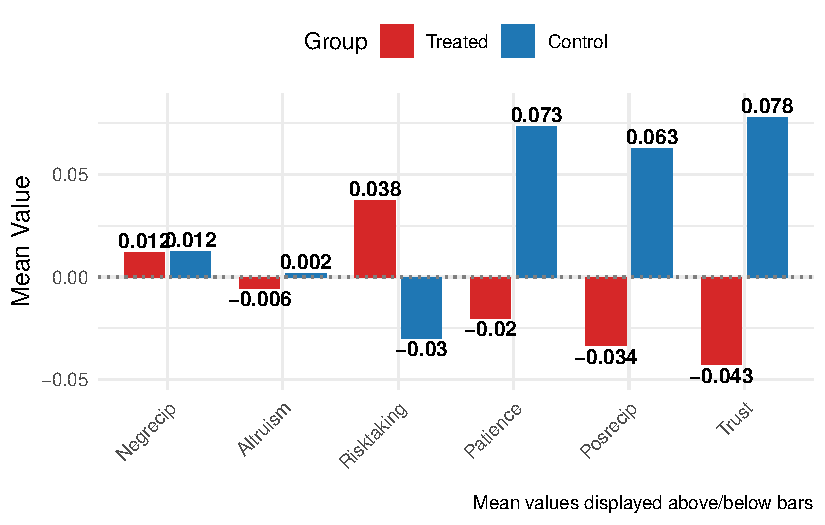
\includegraphics{Milestone-2-Data_files/figure-pdf/fig-a-1.pdf}

}

\caption{\label{fig-a}Mean Preference Profiles by Regime Change
Exposure}

\end{figure}

In the Figure~\ref{fig-a} you can see simple mean comparison graph
between Treated and Control group for all 6 economic preferences.For
completeness, we include \textbf{summary statistics} table for all 6
economic preferences in Table~\ref{tbl-preferences}.
Table~\ref{tbl-controls} depicts the summary statistics for our control
variables.

\hypertarget{tbl-preferences}{}
\begin{table}
\caption{\label{tbl-preferences}Economic Preferences Comparison by Group }\tabularnewline

\centering
\begin{threeparttable}
\begin{tabular}[t]{>{\raggedright\arraybackslash}p{2.5cm}>{\centering\arraybackslash}p{2cm}>{\centering\arraybackslash}p{2cm}>{\centering\arraybackslash}p{2cm}}
\toprule
\multicolumn{1}{c}{ } & \multicolumn{3}{c}{Mean (SD)} \\
\cmidrule(l{3pt}r{3pt}){2-4}
 & Control Group & Treatment Group & Difference\\
\midrule
Trust & 0.078
(0.983) & -0.043
(1.001) & -0.121***
(0.008)\\
Patience & 0.073
(1.046) & -0.020
(0.982) & -0.094***
(0.008)\\
Risk Taking & -0.030
(1.014) & 0.038
(0.988) & 0.067***
(0.008)\\
Positive Reciprocity & 0.063
(0.973) & -0.034
(1.012) & -0.096***
(0.008)\\
Negative Reciprocity & 0.012
(0.982) & 0.012
(1.001) & -0.000
(0.008)\\
\addlinespace
Altruism & 0.002
(1.007) & -0.006
(0.990) & -0.007
(0.008)\\
\bottomrule
\end{tabular}
\begin{tablenotes}
\item \textit{Note:} 
\item Standard deviations in parentheses. Standard errors for differences in parentheses.
\item[*] *** p<0.001, ** p<0.01, * p<0.05, + p<0.1
\end{tablenotes}
\end{threeparttable}
\end{table}

\hypertarget{tbl-controls}{}
\begin{table}
\caption{\label{tbl-controls}Control Variables Comparison by Group }\tabularnewline

\centering
\begin{threeparttable}
\begin{tabular}[t]{>{\raggedright\arraybackslash}p{2.5cm}>{\centering\arraybackslash}p{2cm}>{\centering\arraybackslash}p{2cm}>{\centering\arraybackslash}p{2cm}}
\toprule
\multicolumn{1}{c}{ } & \multicolumn{3}{c}{Mean (SD)} \\
\cmidrule(l{3pt}r{3pt}){2-4}
 & Control Group & Treatment Group & Difference\\
\midrule
age & 43.768
(16.132) & 40.341
(17.763) & -3.427***
(0.129)\\
gdppc_2012 & 22873.619
(16970.573) & 16286.720
(13699.832) & -6586.899***
(123.711)\\
Subjective Math Skills & 5.342
(2.795) & 5.132
(2.813) & -0.210***
(0.022)\\
\bottomrule
\end{tabular}
\begin{tablenotes}
\item \textit{Note:} 
\item Standard deviations in parentheses. Standard errors for differences in parentheses.
\item[*] *** p<0.001, ** p<0.01, * p<0.05, + p<0.1
\end{tablenotes}
\end{threeparttable}
\end{table}

The Figure~\ref{fig-b} below depict the average values grouped by
country in \emph{2012} and \emph{2013}.

\begin{figure}[H]

{\centering 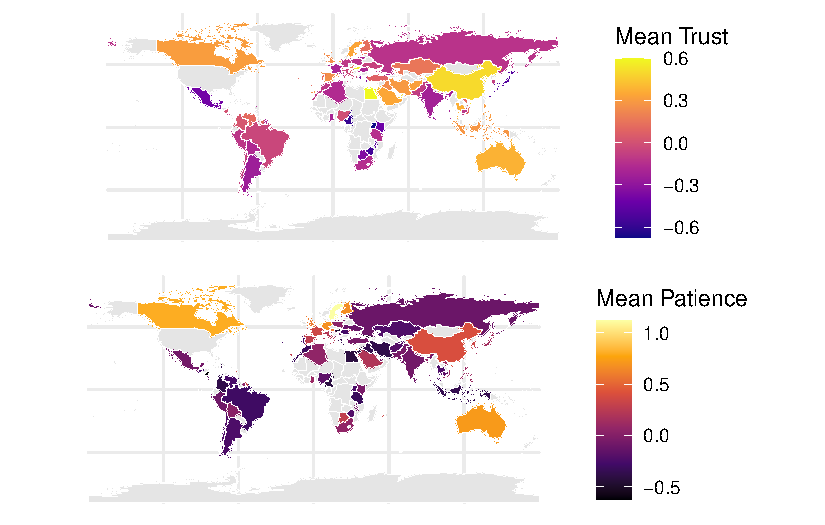
\includegraphics{Milestone-2-Data_files/figure-pdf/fig-b-1.pdf}

}

\caption{\label{fig-b}Average Economic Preference Values by Country}

\end{figure}

\hypertarget{descriptive-statistics}{%
\section{\texorpdfstring{\textbf{Descriptive
statistics}}{Descriptive statistics}}\label{descriptive-statistics}}

The following figures present a detailed \textbf{visual overview of the
descriptive statistics}, including distribution histograms, group-level
comparisons, and difference-in-differences style visualizations
highlighting trends across cohorts.

\begin{figure}[H]

{\centering 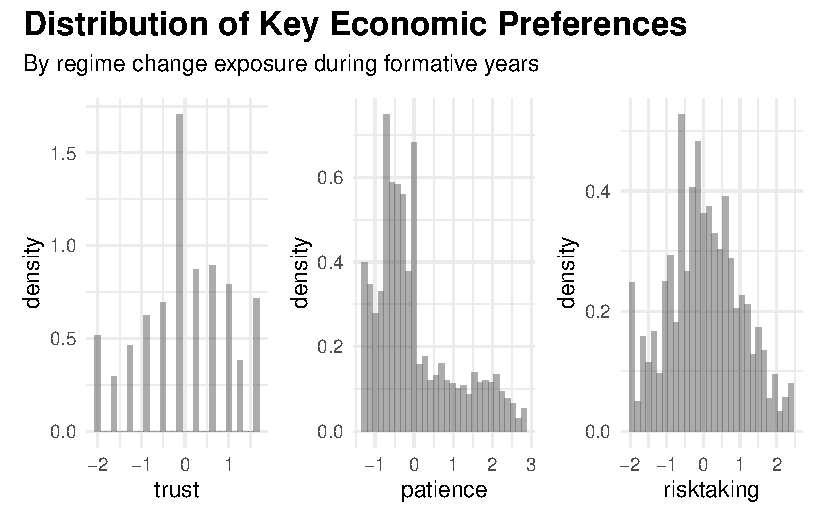
\includegraphics{Milestone-2-Data_files/figure-pdf/fig-c-1.pdf}

}

\caption{\label{fig-c}Distribution of Key Economic Preferences}

\end{figure}

The following figures present additional visualizations of our data. In
the following two graphs we are aiming to evaluate the \textbf{parallel
trends assumption}.

The patience graph shows largely parallel trends for middle-aged groups
(30-65), supporting the DiD assumption for these cohorts. A notable
divergence appears in older ages (65+), where the no-regime-change group
shows sharp decline while the regime-change group remains stable,
suggesting potential long-term protective effects of early regime
exposure on patience.

The trust graph reveals consistently higher trust levels among those
without regime change experience across most age groups.The significant
trust gap in youngest cohorts (15-25) provides some evidence supporting
the hypothesis that experiencing regime changes during formative years
negatively impacts trust development. Interestingly, this gap narrows
and even reverses in the oldest cohorts (65+), suggesting possible
delayed resilience effects.

\begin{figure}[H]

{\centering 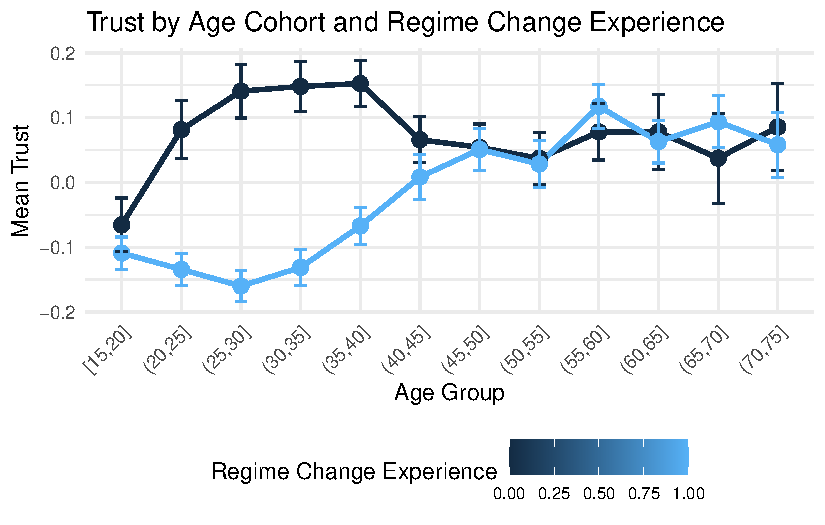
\includegraphics{Milestone-2-Data_files/figure-pdf/unnamed-chunk-3-1.pdf}

}

\end{figure}

\begin{figure}[H]

{\centering 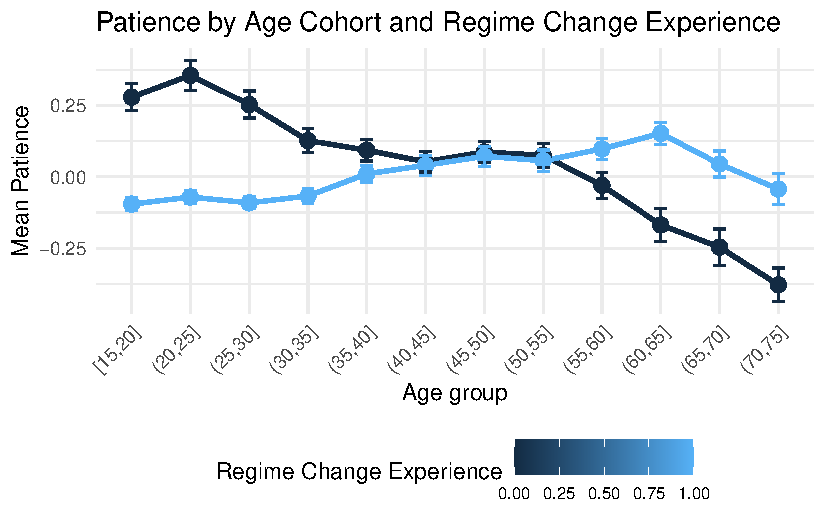
\includegraphics{Milestone-2-Data_files/figure-pdf/unnamed-chunk-3-2.pdf}

}

\end{figure}

\begin{verbatim}
`geom_smooth()` using formula = 'y ~ x'
\end{verbatim}

\begin{verbatim}
Warning: The following aesthetics were dropped during statistical transformation:
colour.
i This can happen when ggplot fails to infer the correct grouping structure in
  the data.
i Did you forget to specify a `group` aesthetic or to convert a numerical
  variable into a factor?
\end{verbatim}

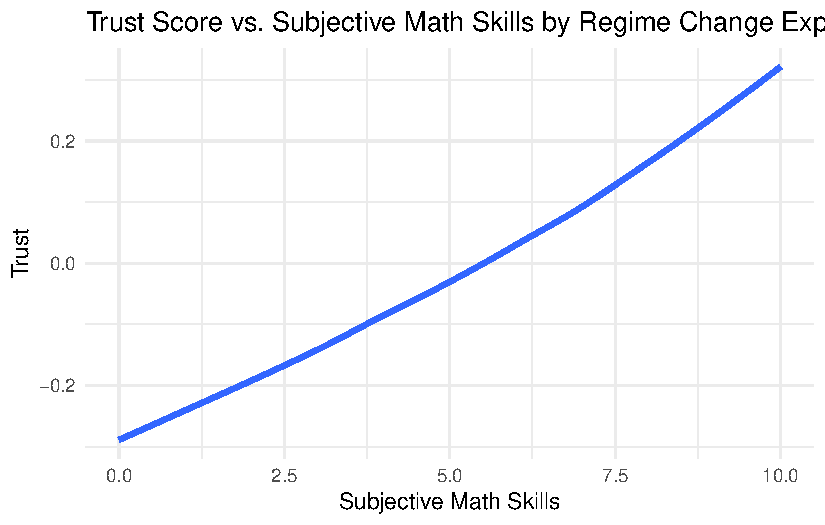
\includegraphics{Milestone-2-Data_files/figure-pdf/unnamed-chunk-4-1.pdf}

\hypertarget{list-of-tables}{%
\section{List of Tables}\label{list-of-tables}}

\hypertarget{references}{%
\section{\texorpdfstring{\emph{References}}{References}}\label{references}}

\hypertarget{refs}{}
\begin{CSLReferences}{1}{0}
\leavevmode\vadjust pre{\hypertarget{ref-balasundaram2025}{}}%
Balasundaram, Palanikumar, and Indirapriya Darshini Avulakunta. 2025.
{``Human Growth and Development.''} In. Treasure Island (FL): StatPearls
Publishing. \url{http://www.ncbi.nlm.nih.gov/books/NBK567767/}.

\leavevmode\vadjust pre{\hypertarget{ref-bolt_maddison-style_2025}{}}%
Bolt, Jutta, and Jan Luiten van Zanden. 2025. {``Maddison-Style
Estimates of the Evolution of the World Economy: A New 2023 Update.''}
\emph{Journal of Economic Surveys} 39 (2): 631--71.
\url{https://doi.org/10.1111/joes.12618}.

\leavevmode\vadjust pre{\hypertarget{ref-coppedge_v-dem_2025}{}}%
Coppedge, Michael, John Gerring, Carl Henrik Knutsen, Staffan I.
Lindberg, Jan Teorell, David Altman, Fabio Angiolillo, et al. 2025.
{``V-Dem Dataset V15.''} Varieties of Democracy (V-Dem) Project.
\url{https://doi.org/10.23696/VDEMDS25}.

\leavevmode\vadjust pre{\hypertarget{ref-detlefsen_are_2024}{}}%
Detlefsen, Lena, Andreas Friedl, Katharina Lima de Miranda, Ulrich
Schmidt, and Matthias Sutter. 2024. {``Are Economic Preferences Shaped
by the Family Context? The Relation of Birth Order and Siblings' Gender
Composition to Economic Preferences.''} \emph{Journal of Risk and
Uncertainty} 69 (1): 1--31.
\url{https://doi.org/10.1007/s11166-024-09433-7}.

\leavevmode\vadjust pre{\hypertarget{ref-falk_global_2018}{}}%
Falk, Armin, Anke Becker, Thomas Dohmen, Benjamin Enke, David Huffman,
and Uwe Sunde. 2018. {``Global Evidence on Economic Preferences.''}
\emph{The Quarterly Journal of Economics} 133 (4): 1645--92.
\url{https://doi.org/10.1093/qje/qjy013}.

\leavevmode\vadjust pre{\hypertarget{ref-luhrmann_autocratization_2020}{}}%
Lührmann, Anna, and et al. 2020. {``Autocratization Surges -- Resistance
Grows.''} V-Dem Institute.
\url{https://www.v-dem.net/media/publications/dr_2020.pdf}.

\end{CSLReferences}



\end{document}
